\documentclass{article} 
\usepackage{beamerarticle}

%\documentclass[ignorenonframetext]{beamer} 
%\usetheme{Warsaw}
%\usepackage{lipsum}


\usepackage{hyperref}
\usepackage[references,links]{agda}
\usepackage{amsmath}
\usepackage{amsthm}
\usepackage{mathtools}
\usepackage{textgreek}
\usepackage{catchfilebetweentags}
\usepackage{tipa}
\usepackage{graphicx}
\usepackage{bussproofs}
\usepackage{tikz}
\usepackage{parskip}

%math
\newcommand{\alp}{\ensuremath{\alpha}}
\newcommand{\lamb}{\ensuremath{\lambda}}
\newcommand{\alpsym}{\ensuremath{\sim_\alpha}}
\newcommand{\choice}{\ensuremath{\chi}}
\newcommand{\p}{\ensuremath{\rightrightarrows}}
\newcommand{\pn}{\ensuremath{\rightrightarrows_n}}
\newcommand{\ninb}{\ensuremath{\not\in_b}}
\newcommand{\inb}{\ensuremath{\in_b}}
\newcommand{\bvc}{\textbf{bvc}}

%Agda
\newcommand{\freshin}[2]{\ensuremath{#1 \mathbin{\AgdaDatatype{\#}} #2}}
\newcommand{\lambAg}[2]{\ensuremath{\AgdaInductiveConstructor{ƛ}\, #1\, #2}}
\newcommand{\inAg}{\ensuremath{\mathbin{\AgdaFunction{∈}}}}
\newcommand{\ninAg}{\ensuremath{\mathbin{\AgdaFunction{∉}}}}
\newcommand{\neqAg}{\ensuremath{\mathbin{\AgdaInductiveConstructor{≢}}}}
\newcommand{\ap}[2]{#1 \ensuremath{\mathbin{\AgdaInductiveConstructorFunction{·}} #2}}
\newcommand{\var}[1]{\ensuremath{\AgdaInductiveConstructorFunction{v}\, #1}}
\newcommand{\fv}{\ensuremath{{\AgdaFunction{fv}}\,}}
\newcommand{\perm}{\ensuremath{\mathbin{\AgdaFunction{∙}}}}
\newcommand{\perma}{\ensuremath{\mathbin{\AgdaFunction{∙}_a}}}
\newcommand{\free}{\ensuremath{\mathbin{\AgdaFunction{*}}}}
\newcommand{\choiceAg}{\ensuremath{\AgdaFunction{χ}\,}}
\newcommand{\choiceAgaux}{\ensuremath{\AgdaFunction{χ'}\,}}
\newcommand{\alpeqAg}{\ensuremath{\mathbin{\AgdaDatatype{∼α}}}}
\newcommand{\swap}[3]{\ensuremath{(#1 \mathbin{\AgdaFunction{∙}} #2)\, #3}}

\newcommand{\betaalpha}{\ensuremath{\rightarrow_\alpha}}
\newcommand{\f}{\ensuremath{\rightarrow}}
\newcommand{\betaaster}{\ensuremath{\rightarrow_\beta^*}}
\newcommand{\lam}{\ensuremath{\lambda}}
\newcommand{\conc}{\ensuremath{\mathop{+\!\!+}}}


% \newcommand{\agdaf}[1]{\ensuremath{\AgdaFunction{#1}\,}}
% \newcommand{\agdaD}[1]{\ensuremath{\AgdaDatatype{#1}\,}}
% \newcommand{\agdav}[1]{\ensuremath{\AgdaBound{#1}\,}}

\DeclareUnicodeCharacter{411}{\textipa{\textcrlambda}}
\DeclareUnicodeCharacter{65288}{(}
\DeclareUnicodeCharacter{65289}{)}
\DeclareUnicodeCharacter{8788}{\ensuremath{\coloneqq}}
\DeclareUnicodeCharacter{8336}{\ensuremath{_a}}
\DeclareUnicodeCharacter{8799}{\ensuremath{\overset{?}{=}}}
\DeclareUnicodeCharacter{8759}{\ensuremath{\dblcolon}}
\DeclareUnicodeCharacter{8718}{\ensuremath{\square}}

\newtheorem{lem}{Lemma}

\title{Parallel Reduction}

\begin{document}
\maketitle

\section{Barendregt}

Next we extract from page 26 of~\cite{barendregt81} the following variable convention and definitions.

\subsection{BVC Convention}

\subsubsection*{2.1.12 Convention}

Terms that are \alp-congruent are identified.

\subsubsection*{2.1.13 Variable Convention}

If $M_1, \dots M_n$ occur in certain mathematical context, then in these terms all bound variables are chosen to be different from the free variables.


\subsubsection*{2.1.12 Substitution Definition} \label{sec:substitutionBarendregt}

\[
  \begin{array}{llcll}
    x &[x:=N] & \equiv & N &\\
    y &[x:=N] & \equiv & y & \text{if}\ x \not\equiv y\\
    (M_1 M_2) &[x:=N]& \equiv & (M_1 [x:=N]) (M_2 [x:=N]) &\\
    (\lam y . M_1) & [x:=N] & \equiv & \lam y . (M_1 [x:=N])&\\
  \end{array}
\]

\label{notefourth} In the fourth clause it is not needed to say ``provided that $y \not\equiv x$\ and $y \not\in fv(N)$''. By the variable convention this is the case.

There exist subtleties in the use of variable convention. We show next one example of these caused by the composite use of it in the next results.


\subsubsection*{2.1.16 Substitution Composition Lemma}

If $x \not\equiv y$\ and $x \not\in fv(L)$ then:

\[ M [x:=N][y:=L] \equiv M[y:=L][x:=N[y:=L]] \]

Proof: By induction on $M$.
\begin{itemize}
\item{Case 1} $M$ is a variable.
  \begin{itemize}
  \item{Sub-Case 1.2} $M \equiv y$. Then both sides equal L, for $x \not\in fv(L)$ implies $L[x:=\dots]\equiv L$.
    To prove $x \not\in fv(L)$ implies $L[x:=\dots]\equiv L$\ we need to make use of the variable convention with context $x,L$, by doing so we get that $x \ninb L$. We next show that this premise is necessary in the abstraction case of an induction over $L$.

\begin{itemize}
\item Abstraction case : $x \not\in fv(\lam y . M) \Rightarrow (\lam y . M)[ x := N] \equiv \lam y . M$.
  \[\begin{array}{ll}
      (\lam y . M)[ x := N] & \equiv \text{by BVC we can assume } y \not\equiv x \text{ and } y \not\in fv(N) \\
      \lam y . (M [ x := N]) & \equiv \text{by i.h. using } x \not\in fv(M), \text{as } x \not\in fv(\lam y . M) \text{ and } y \not\equiv x \\
      \lam y . M
  \end{array}\]
\end{itemize}

  \end{itemize}
\item{Case 2} $M \equiv \lamb z . M_1$. Again using BVC we may assume that $z \not\equiv x$\ and $z \not\in fv(N,L)$.
\[ \begin{array}{rl}
     (\lam z. M_1)[x:=N][y:=L]      & \equiv  \{z \not\equiv x, y \text{ and } z \not\in fv(N,L) \text{ no capture}\} \\
     \lam z . M_1[x:=N][y:=L]       & \equiv  \{\text{i.h. as } x \not\equiv y, x \not\in fv(L) \} \\
     \lam z . M_1[y:=L][x:=N[y:=L]] & \equiv  \\
     (\lam z . M_1) [y:=L][x:=N[y:=L]] & \\
  \end{array}\]

  So we need the BVC convention holds under the context $x,y,M,N,L$\ in this sub-case.
\end{itemize}


We can conclude, recollecting the uses of BVC from previous proof sub-cases, that substitution composition lemma needs that the BVC hold in the context of $x,y,M,N,L$.

Previus result is used inside the 1.2 sub-case of substitution composition lemma proof (page 60 of~\cite{barendregt81}). We show that the freshness context of previous result can not be obtained inside the proof of next lemma.

\subsubsection*{3.2.4 Substitution preserves parallel relation.}

      \[ M \p M' , N \p N' \Rightarrow M [x:=N] \p M'[x:=N'] \]

By induction on the relation, we show the next problematic sub-case.

\begin{itemize}
\item{Case 4.} $M \p M' \equiv (\lam y. P)Q \p P'[y:=Q']$\ as a direct consequence of $P \p P'$, $Q \p Q'$.
  \[\begin{array}{ll}
      ((\lam y. P)Q) [x:=N] & \equiv \text{by BVC } y \not\equiv x \text{ and } y \not\in fv(N) \\
      (\lam y. (P [x:=N]))(Q [x:=N])  & \p \text{by i.h. and applying a parallel reduction step} \\
      P'[x:=N'][y := Q'[x:=N']  & \equiv \text{by substitution composition lemma 2.1.16} \\
      P'[y:=Q'][x:=N']
  \end{array}\]
\end{itemize}

The first use of BVC can be obtained requiring as BVC context $x,N,M$. But substitution composition lemma needs $y,x,P',Q',N'$ as BVC context. $x,P',Q',N'$\ context could be derived from the context $x,M,N$, as parallel reduction does not create bound neither free variables, thus BVC is preserved, but $y$ is a bound variable of $M$ and so we can not put it in the BVC context of this proof. This problematic use of BVC can not be easily fixed. A fresh variable rename can be done, using \alp-congruent are identified, but then, as we are in a relation induction, the inductive hypothesis will not hold over the renamed sub-term, perhaps we can prove that the relation is preserved by such renamings as an auxiliary lemma, eventhough  this proof can not be fixed in a simple manner. Furthermore, an induction on terms, or even in the length of terms, can not be done because of rule $M \p M$. 

One way to fix this problem is to add to the BVC convention that all bound variables are distinct, by doing so we can know that the bound variable $y$\ does not occur bind in the context $x,P',Q',N'$, then we can deduce that the free variables will not occur bind in the BVC context $x,y,P',Q',N'$ inside the previous proof sub-case.
Norrish rule induction ...

In~\cite{Hindley:2008}, Hindley suggests in lemma 1.20 that we can work removing BVC precondition and replacing term's identity by \alp-equivalence relation, and all theorems will stay true. This work follow this idea up to Church-Rosser theorem. For this, we will introduce the BVC normalising \bvc\ function, and then we will prove several classic results under BVC premise and as pen-and-paper proof. Finally, we will remove the BVC premise to prove the confluence of the parallel reduction relation.

\section{BVC Term Function}

\[
  \bvc : \Lambda \f \Lambda, \text{such that:} \left\{
    \begin{array}{l}
      (\bvc\ M) \alpsym M \\
      M \alpsym N \Rightarrow \bvc\ M \equiv \bvc\ N  \\
      fv (M) \equiv fv(\bvc\ M)  \ninb \bvc\ M \\
      \text{bound variables in } \bvc\  M \text{ are all distinct} \\
  \end{array} \right.
\]

Given any term, this function returns an \alp-equivalent one, but satisfiying the BVC convention. As previously explained, we will add to the BVC that all bound variables are different. We already explained this addition in the context of a particular proof. But now we argue that this addition is intuitive, trying to justiy that its addition is neccessary in general.

To reason as in informal practice, the third and fourth properties should be preserved over terms induction, and also through relations over terms. For this, we show next that the third property alone is not enough in the abstraction case of an induction over terms. So with premise $fv (\lam x. M) \ninb \lam x .M$\ we need to prove that $fv(M) \ninb M$. By free variables function definition $fv (M) - \{ x \}  \ninb \lam x .M$, thus using $\ninb$\ definition, $fv (M) - \{ x \}  \ninb M$. In the case that $x \in fv(M)$, we can not get the desired result because we can not infer $x \ninb M$, which can be derived if we assume the fourth premise also holds, as if all binders not equal in $\lam x . M$\ then $x \ninb M$.

\section{Parallel Reduction}\label{parallel}

Naive parallel reduction, almost identical to Barendregt ones but replacing $M \p M$\ rule by $x \p x$ one. Note that naive substitution is used in the last rule, implemented as a direct fold and equivalent to Barendregt's substitution definition~\ref{sec:substitutionBarendregt}.

\begin{minipage}{0.25\linewidth}
  \AxiomC{$$}   \LeftLabel{\pn v} \UnaryInfC{$x \pn x$} \DisplayProof
\end{minipage}
\begin{minipage}{0.45\linewidth}
  \AxiomC{$M \pn M'$} 
  \AxiomC{$N \pn N'$}
  \LeftLabel{\pn a}
  \BinaryInfC{$M N \pn M' N'$} \DisplayProof
\end{minipage}
\begin{minipage}{0.25\linewidth}
  \AxiomC{$ M \pn N$} 
  \LeftLabel{\pn \lam}
  \UnaryInfC{$\lambda x M  \pn  \lambda x N$} \DisplayProof
\end{minipage}

\begin{center}
  \AxiomC{$M \pn M'$}
  \AxiomC{$N \pn  N'$}
  \LeftLabel{$\pn \beta$}
  \BinaryInfC{$(\lambda x M) N  \pn M' [x := N']_n$}
  \DisplayProof
\end{center}

We can prove substitution composition lemma 3.2.4 in a similar way to Barendregt work, but adding all bound variables are distinct to fix previously explained problem.

As common practice when proving the confluence property of the parallel relation, we introduce the function that recursively reduces all $\beta$-redexes in a term.

  \[
  \begin{array}{llll}
    x &&^* &= x \\
    (\lam x . M)&&^* &= \lam x . M^* \\
    (x &M)&^* &= x M^*  \\
    ((M_1 M_2) & M_3)&^* &= (M_1 M_2)^* M_3^* \\
    ((\lam x . M_1) & M_2)&^* &= M_1^* [x := M_2^*]_n 
  \end{array} 
  \]

  Using the substitution composition lemma we can prove that, under the BVC convention with context $M$, $M \pn N \Rightarrow N \pn M^*$ holds. The proof is a direct induction on $M$ term, except from the next application sub-case.

  \begin{itemize}
  \item{Application $M \equiv (\lam x . M) N$, $\pn \beta$\ sub-case. }

    \begin{minipage}{0.5\linewidth}
    Hypotheses:
      \AxiomC{$M \pn M'$}
      \AxiomC{$N \pn  N'$}
      \LeftLabel{$\pn \beta$}
      \BinaryInfC{$(\lambda x M) N  \pn M' [x := N']_n$}
      \DisplayProof
  \end{minipage}
  \begin{minipage}{0.5\linewidth}
    Thesis: \[ M' [x := N']_n \pn  \underbrace{((\lambda x M) N)^*}_{=M^* [x := N^*]_n}\]
  \end{minipage}
  Proof:
  \AxiomC{$M \pn M'$}
  \LeftLabel{ih}
  \UnaryInfC{$M' \pn M^*$}
  \AxiomC{$N \pn  N'$}
  \LeftLabel{ih}
  \UnaryInfC{$N' \pn N^*$}
  \LeftLabel{3.2.4 lemma}
  \BinaryInfC{$M' [x := N']_n \pn  M^* [x := N^*]_n$}
  \DisplayProof


  
  The application of 3.2.4 lemma in previous proof tree requires the BVC context $x,M',N'$, which can be derived from knowing BVC holds for $(\lambda x M) N$\ and that \pn\ relation preserves the BVC convention. Again, here is essential that binder are all different in the BVC context.
\end{itemize}

From this result it is directly derived that \pn\ has diamond property. Also we can prove it is invariant by a simple term induction.

Next lemma establish that the introduced relation is independant from variable binders choices, under BVC conditions to ensure that the naive substitution can be correctly applied inside $\pn\beta$ relation rule. In other words, this lemma says that every parallel reduction can be reproduced for any \alp-equivalent term  satisfing the BVC condition.

\begin{lemma}{Naive parallel reduction can be reproduced for BVC \alp-equivalent terms.} \label{lemma:parallelrenaming}

  \begin{minipage}{0.75\linewidth}
  \[ BVC\ M, BVC\ M', M \pn N \Rightarrow \exists N', N  \alpsym N', M' \pn N' \]
\end{minipage}
\begin{minipage}{0.25\linewidth}
  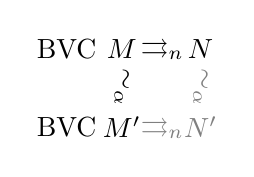
\begin{tikzpicture}[>=latex]
   \node (M) at (0,1) {$M$};
   \node (BVCM) at (-0.7,1) {BVC};
   \node (M') at (0,0) {$M'$};
   \node (BVCM') at (-0.7,0) {BVC};
   \node (N) at (1,1) {$N$};
   \node[opacity=0.5] (N') at (1,0) {$N'$};

   \path               (M) --node{\pn} (N);
   \path [opacity=0.5,->] (M') --node{\pn} (N') ;
   \path               (M) --node[sloped]{$\alpsym$} (M');
   \path [opacity=0.5] (N) --node[sloped]{$\alpsym$} (N');
\end{tikzpicture}
\end{minipage}
\end{lemma}

\begin{proof}
   
\end{proof}

In a proof assistant we can not identify \alp-compatible terms as the BVC convention does, so we need to introduce the following proper parallel relation definition over the \alp-equivalence classes of terms.

\begin{definition}{Parallel Reduction}
\begin{minipage}{0.7\linewidth}
\[ M \p N \equiv \exists N', \bvc\ M \pn N' , N' \alpsym N \]
\end{minipage}
\begin{minipage}{0.30\linewidth}
  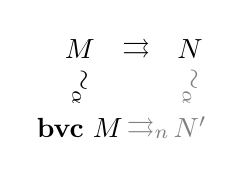
\begin{tikzpicture}[>=latex]
   \node (M) at (0,1) {$M$};
   \node (bvcM) at (0,0) {$\bvc\ M$};
   \node (N) at (1.4,1) {$N$};
   \node[opacity=0.5] (N') at (1.4,0) {$N'$};

   \path               (M) --node{\p} (N);
   \path [opacity=0.5,->] (bvcM) --node{\pn} (N') ;
   \path               (M) --node[sloped]{$\alpsym$} (bvcM);
   \path [opacity=0.5] (N) --node[sloped]{$\alpsym$} (N');
\end{tikzpicture}
\end{minipage}
\end{definition}

This relation is left and right \alp-compatible. Now we prove the diamond property of \p.

\begin{theorem}{\p\ has diamond property}

  \begin{minipage}{0.7\linewidth}
  \[ M \p N, M \p P \Rightarrow \exists R, N \p R, P \p R \]
\end{minipage}
  \begin{minipage}{0.3\linewidth}
  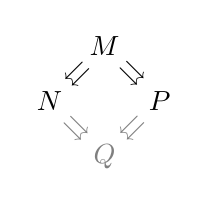
\begin{tikzpicture}[>=latex]
   \node (M) at (0.7,0.7) {$M$};
   \node (N) at (0,0) {$N$};
   \node (P) at (1.4,0) {$P$};
   \node[opacity=0.5] (Q) at (0.7,-0.7) {$Q$};

   \path               (M) --node[sloped, auto=false, allow upside down]{\p} (N);
   \path               (M) --node[sloped, auto=false, allow upside down]{\p} (P) ;
   \path [opacity=0.5] (N) --node[sloped, auto=false, allow upside down]{\p} (Q);
   \path [opacity=0.5] (P) --node[sloped, auto=false, allow upside down]{\p} (Q);
\end{tikzpicture}
\end{minipage}

\end{theorem}

\begin{proof}
  Hypotheses: Be $M' \equiv \bvc\ M, N'' = \bvc\ N, P'' = \bvc\ P$ then:
    \begin{align}
    M \p N \equiv \exists N', &M' \pn N' , N' \alpsym N \label{theorem:confluencehi1}\\
    M \p P \equiv \exists P', &M' \pn P' , P' \alpsym P \label{theorem:confluencehi2}
      \end{align}\label{theorem:confluence}


      \begin{center}
  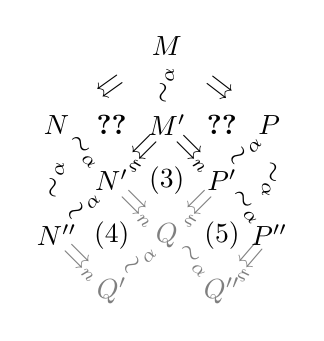
\begin{tikzpicture}[>=latex]

   \node (M) at (0.7,1.7) {$M$};
   \node (M') at (0.7,0.7) {$M'$};
   \node (1) at (0,0.7) {$\ref{theorem:confluencehi1}$};
   \node (2) at (1.4,0.7) {$\ref{theorem:confluencehi2}$};
   \node (3) at (0.7,0) {$(3)$};
   \node (N') at (0,0) {$N'$};
   \node (N'') at (-0.7,-0.7) {$N''$};
   \node (4) at (0,-0.7) {$(4)$};
   \node (N) at (-0.7,0.7) {$N$};
   \node (P') at (1.4,0) {$P'$};
   \node (P) at (2,0.7) {$P$};
   \node (P'') at (2,-0.7) {$P''$};
   \node[opacity=0.5] (Q) at (0.7,-0.7) {$Q$};
   \node (5) at (1.4,-0.7) {$(5)$};
   \node[opacity=0.5] (Q') at (0,-1.4) {$Q'$};
   \node[opacity=0.5] (Q'') at (1.4,-1.4) {$Q''$};


   \path [opacity=0.5] (Q) --node[sloped]{\alpsym} (Q');
   \path [opacity=0.5] (Q) --node[sloped]{\alpsym} (Q'');


   \path [opacity=0.5] (N'') --node[sloped]{\pn} (Q');
   \path [opacity=0.5] (P'') --node[sloped]{\reflectbox{\pn}} (Q'');

   \path               (M') --node[sloped]{\alpsym} (M);
   \path [opacity=0.5] (N') --node[sloped]{\pn} (Q);
   \path [opacity=0.5] (P') --node[sloped]{\reflectbox{\pn}} (Q);

   \path               (N'') --node[sloped]{\alpsym} (N);
   \path               (N'') --node[sloped]{\alpsym} (N');
   \path               (N) --node[sloped]{\alpsym} (N');

   \path               (P) --node[sloped]{\alpsym} (P');
   \path               (P'') --node[sloped]{\alpsym} (P');
   \path               (P) --node[sloped]{\alpsym} (P'');
   \path               (M) --node[sloped,  allow upside down]{\p} (N);
   \path               (M') --node[sloped]{\reflectbox{\pn}} (N');
   \path               (M') --node[sloped, auto=false, allow upside down]{\pn} (P');
   \path               (M) --node[sloped, auto=false, allow upside down]{\p} (P) ;
 \end{tikzpicture}
      \end{center}

  $M'$\ satisfies the BVC convention so we can apply diamond property of \pn\ to infer the inner diamond $(3)$\ in previous image, that is, there exist $Q$\ such that $N' \pn Q$\ and $P' \pn Q$. As \pn\ preserves the BVC convention, $N'$\ and $P'$ satisfies the BVC convention, we can use previous lemma~\ref{lemma:parallelrenaming} to derive $(4)$\ and $(5)$, from which by definition of \p\ $N \p Q$\ and $P \p Q$ hold. 
\end{proof}

\bibliographystyle{alpha}
\bibliography{resumen.bib}


\end{document}